\documentclass[12pt]{article}

\textwidth=6.5in
\textheight=8in
\topmargin=0in
\headheight=0.50in
\headsep=0.0in
\footskip=0.5in
\oddsidemargin=0in
%\pagestyle{headings}
\usepackage{graphicx}
\usepackage{hyperref}
\usepackage{listings}
\usepackage{amsmath}



\begin{document}

\tableofcontents

\section{Introduction}

Three items are presented here. The first is an algorithmic description of the back-propagation process, used to nudge the weights and biases of a neural network so that inputs to the network produce desired outputs to within some arbitrarily small error. This intended for those  wishing to hand-code their own neural network with back propagation, and need the associated logic and equations to do so. 

This initial presentation is focused on building yourself an 'instructive' neural network, where each neuron is actually a structure containing its own input, activation, delta, and an array of weights that connects it to the neurons in the next forward layer. For this,  pseudo-code is presented indicating how both forward and backward passes through such a a neural network work.  Such a neural network is not meant to be fast or 'production ready' (in fact, it's quite slow), but is nonetheless instructive.

The second is a matrix representation of the same. This allows for the use of a matrix library such as Numpy to speed up the calculations required of the neural network.

The third is a ``calculus first'' derivation of the equations that drive back-propagation. The calculus-first derivation keeps the logic clean by relying only on the chain and product rules of calculus, with simplifications of the results that require a thoughtful interpretation of the internal properties of a neural network.



\section{Motivation: Develop an educational neural network}

The goal of this work is to develop an ``educational'' neural network that  can be used to understand how back propagation works.  By educational we mean there won't be any optimizations, matrices, or linear algebra. The network will run with nested for-loops and really obvious variable names.  Back propagation equations will just be stated as givens and used as such.  In this educational model, a data structure will be developed for a neuron that will contain information an individual neuron needs to hold, and  see how it connects to the larger network.  The result will be a complete neural network that you can train and use, but it'll be slow.

\subsection{A neuron data structure}

In this work the educational neural network was developed in Python.  Each neuron is represented by a Python dictionary that looks like this:

\begin{lstlisting}[language=Python,
		basicstyle=\small\ttfamily,
                 numbers=left,
                 stepnumber=1,
                 numbersep=8pt,
                 tabsize=2,
                 showspaces=false,
                 breaklines=true,
                 showstringspaces=false,
                 columns=fullflexible]
 {
    "desc": desc,
    "z":0.0,        	#input
    "a": 0.0,       	#activation
    "b": 0.01,       #bias
    "w": [],     	#weights
    "delta": 0.0
}
\end{lstlisting}
Here {\tt z}, {\tt a}, and {\tt b} are the neuron's input, activation and bias. The {\tt w} is a list of  initially small random numbers representing each weight that connects this neuron to the neurons in the next forward layer. If for example, the forward layer has $6$ neurons in it, this list will contain $6$ floating point values. Lastly, the {\tt delta} is the ``error'' of the neuron's output, which is used in the back propagation process.

A layers of neurons is represented as a list of this basic neuron structure, with one structure per neuron in a layer.  A similar implementation in C would likely use a {\tt struct} to define a neuron. 



\subsection{Definitions}
\label{definitions}

The neural network (or a section of a larger network) analyzed here is shown in Figure~\ref{nn}.  Three alphabetical letters are chosen to refer to the layers, $i$, $j$, and $k$.  The output layer is $k$, which is fed from hidden (or inner) layer $j$, which is fed from another layer $i$. Note $i$ may also be the input layer or another hidden layer.  More layers can be expanded to the left of $i$, perhaps layer $h$ (which is referenced below). 

All neurons between layers are interconnected.  Based on this structure, here are a few definitions used throughout this work (note, we used the generics $x$ and $y$ below, which can refer to $i$, $j$, or $k$).

\begin{figure}[h]
\begin{center}
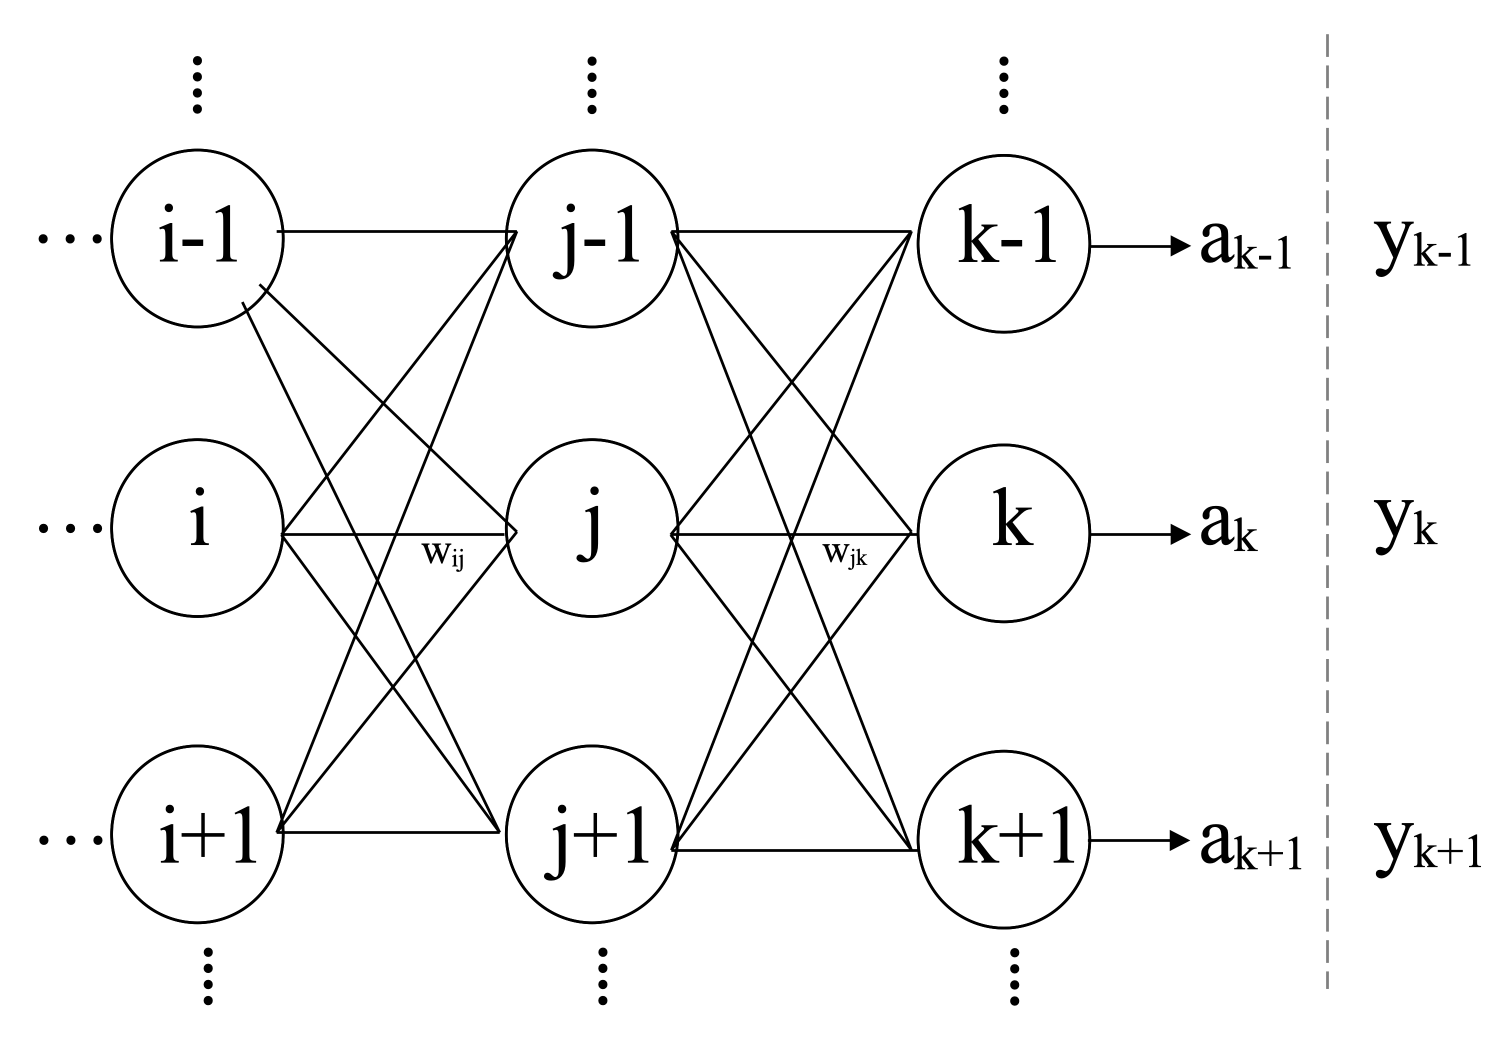
\includegraphics[scale=0.2]{Figs/nn_fig.png}
\caption{The neural network modeled here. The output layer is referenced with the $k$ index and the hidden layers with $j$ and $i$. The weights $w_{ij}$ and $w_{jk}$ are highlighted, as they are used in the text.}
\label{nn}
\end{center}
\end{figure}

\begin{itemize}

\item $w_{xy}$. This refers to the weight of neuron $x$ in layer $L$ into neuron $y$ in layer $L+1$.  This could be expressed as $w_{L,x\rightarrow(L+1),y}$ or $w^{L}_x\rightarrow w^{L+1}_y$, or something similar, but we aim here to simplify the notation. So, $w_{ij}$ will be the weight between the $i^{th}$ neuron in layer $i$ and the $j^{th}$ neuron in layer $j$, with $j=i+1$ (always).  

To simplify notation, $i$, $j$, and $k$ are used to denote both layers and individual neurons.  We hope this balances any conceptual confusion with notational simplicity by the context in which something is mentioned.  So, layer $i$, or neuron $i$ (implied in layer $i$) can be referenced, as can $w_{ij}$ as the weight connecting neuron $i$ (in implied layer $i$) to layer $j$ (in implied layer $j$).

As used here in $w_{xy}$, $x$ is always in a layer that feeds input data forward into the layer that contains neuron $y$, so $y$ is always $x+1$.  In general, $x$ is an index that can run from $1$ to the number of neurons in the layer. In words, $w_{xy}$ would be read ``the weight from neuron $x$ in implied layer $x$ into neuron $y$ in implied layer $y$'' with the implicit meaning that neuron $x$ feeds neuron $y$.  Symbolically, $w_{from-layer\rightarrow to-layer}$.

Note: it turns out that the {\tt from layer}$\rightarrow${\tt to layer} notation may not be good in the long term, as it'll go counter to some numbering conventions used in he matrix representation (see below). The {\tt from layer}$\rightarrow${\tt to layer} idea however, is just too tempting to pass up as we try to grasp back propagation.  We'll point this out again in the matrix treatment, and even point out the same decision made by other authors.

\item $z_{y}$. This is the input to neuron $y$ from the backward (or leftward) layer $x$ that feeds it. Here

\begin{equation}
z_y = \sum_x w_{xy} a_x + b_y.
\label{eqn_zy}
\end{equation}

So,  the input to neuron $y$, or $z_y$, is given by a sum over all of the products of the weights that feed it from layer $x$ $(w_{xy})$ and the activation of the neuron feeding that weight from layer $x$, $a_x$ (see below), plus the bias of the destination neuron, $b_y$ (see below).

\item $f(x)$ is the squashing function or activation function for a neuron, and $f'(x)$ is the derivative of the activation function.  Note, seeing something like $f'(z_k)$ means to find the derivative of $f$ (with respect to its independent variable, $x$ for example) then evaluate the derivative at $z_k$.  $f$ is typically ReLU or the sigmoid function.

\item $a_x$ this is the ``activation'' of neuron $x$, defined as $a_x=f(z_x)$.

\item $y_x$ is the target (or needed) value of an output neuron.  The goal of back propagation is to make all $a_x$ values arbitrarily close to a corresponding $y_x$ value.

\end{itemize}

\subsection{The forward pass}

\subsubsection{Pseudo-code}

Here is pseudo-code that will take an input vector {\tt input} and send it forward through the network.  A few notes on the code:

\begin{enumerate}

\item A neuron is specified in a cartesian $(x,y)$ format like {\tt (neuron,layer)} where {\tt neuron} is the neuron number in layer {\tt layer}.  
\item Any other network-wide variable is in parentheses like {\tt output$\_$layer} which is the numerical index to the output layer (and presumably an array of output layer neurons).
\item All for-loop are inclusive of both their starting and ending values.

\end{enumerate}


\begin{lstlisting}[language=Python,
		basicstyle=\small\ttfamily,
                 numbers=left,
                 stepnumber=1,
                 numbersep=8pt,
                 tabsize=2,
                 showspaces=false,
                 breaklines=true,
                 showstringspaces=false,
                 columns=fullflexible]
#load up input layer
for neuron = 0 to (number of input neurons):
  z of input neuron (neuron) = input vector[neuron]
  a of input neuron (neuron) = f(z of input neuron (neuron))
end
	
#propagate from input layer through the entire network
for layer = 0 to output_layer-1
  forward_layer = layer + 1
  for forward_neuron = 0 to  neuron in layer (forward_layer)
    z = 0.0
    for neuron =0 to count of neurons in layer (layer)
      z = z + weight connecting (layer,neuron) and (forward_layer,forward_neuron) * a of (layer,neuron)  + bias of (layer,neuron)
    end
    z of (forward_layer,forward_neuron) = z
    a of (forward_layer,forward_neuron) = f(z)
  end
end
\end{lstlisting}

\subsection{Back-propagation}

Here we assume you have a set of input/output vectors on which you'd to train the network.  Assuming your output layer is layer $k$, the layer to the left of it is $j$, and to the left of it $i$, here's how to correct the weights via back-propagation. Before beginning, establish some learning rate $\eta$ for the back-propagation.

\begin{enumerate}


\item Send an input vector forward through the network and compute $z_x$ and $a_x=f(z_x)$ for all neurons in the network.

\item For each neuron $k$ in the output layer compute $\delta_k=f'(z_k)(a_k-y_k)$, where $y_k$ is the corresponding component of the output vector.

\item Loop through all weights between layers $j$ and $k$. It's best to loop through $j$ as the outer loop and $k$ and the inner loop.  Correct $w_{jk}$ like this
\begin{equation}
w_{jk,new} = w_{jk,old}-\eta\delta_k a_j.
\end{equation}

\item Loop through all neurons in layer $j$ and compute $\delta_j$ for each neuron from the formula $\delta_j=f'(z_j)\sum_k \delta_k w_{jk}$. It's best to start an outer loop on $j$ through the neurons, an inner loop on $k$ to compute the sum.

\item Loop through all weights between layers $i$ and $j$.  Use $i$ as your outer loop, and $j$ as your inner loop.  Correct $w_{ij}$ like this
\begin{equation}
w_{ij,new} = w_{ij,old}-\eta\delta_j a_i.
\end{equation}

\item \label{bp_loop} Have a layer to the left of $i$? Call it $h$.  Loop through all neurons in layer $i$ and compute $\delta_i$ for each neuron from the formula $\delta_i=f'(z_i)\sum_j \delta_j w_{ij}$.  It's best to start an outer loop on $i$ through the neurons, an inner loop on $j$ to compute the sum.

\item Loop through all weights between layers $h$ and $i$.  Use $h$ as your outer loop, and $i$ as your inner loop.  Correct $w_{hi}$ like this
\begin{equation}
w_{hi,new} = w_{hi,old}-\eta\delta_i a_j.
\end{equation}


\end{enumerate}

You may have more hidden weights to correct, in which case the pattern evolving pattern here can be used. So, instead of continuing with explicit formulas for correcting the rest of your weights, let's come up with a systematic pattern.

Let's suppose the last set of weights you corrected were between layers $b$ and $c$, where $c$ is always $b+1$.  So you corrected weights $w_{bc}$. Now you want to keep going and correct weights $w_{ab}$, where $a$ is $b-1$. Here's what you'd do

\begin{enumerate}

\item Since you corrected weights $w_{bc}$, you must have all of the $\delta_c$ values available.

\item Compute $\delta_b$ from $\delta_b=f'(z_b)\sum_c\delta_c w_{bc}$.	

\item Correct $w_{ab}$ with $w_{ab,new}=w_{ab,old}-\eta(\delta_b a_a)$.

\end{enumerate}

\begin{figure}[h]
\begin{center}
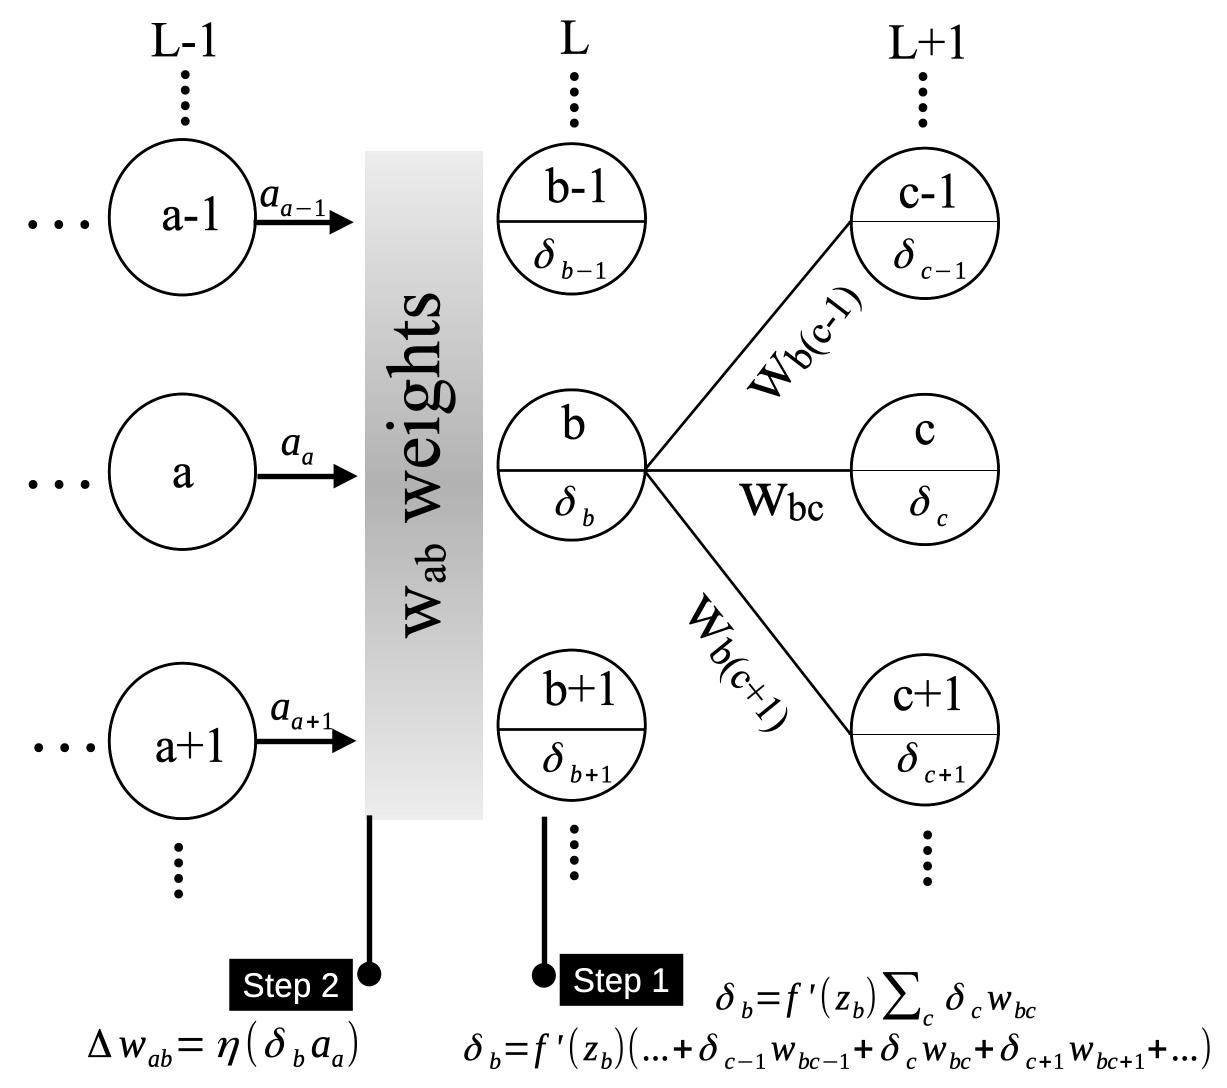
\includegraphics[scale=0.3]{Figs/wxy_change.png}
\caption{The back propagation plan. Step 1: Compute $\delta_j$ for the first layer to the left of the last one that has been corrected (i.e. the last one whose $\delta$s are known). Step 2: Adjust the weights by $\Delta w_{ab}$.}
\label{wxy_change}
\end{center}
\end{figure}


\subsubsection{Pseudo-code}

Here's pseudo code (illustrated in Figure~\ref{wxy_change}) that will traverse a network backward, correcting its weights and neuron biases. The following assumptions are made: 

\begin{enumerate}
\item You have appropriate data structures for a neural network all set up.
\item A forward pass of some input has been applied to the network and all neuron inputs ($z$) and activations $a=f(z)$ have been computed.  
\item You know the corresponding output for a given input.
\item You can retrieve the number of neurons in a given layer, as well as $a$ and $z$ for any neuron.
\item You can retrieve the weight connecting any two neurons and modify it.
\item You can retrieve the bias of a neuron and modify it.
\item You've defined some learning rate {\tt eta} and some learning rate for the biases {\tt eta$\_$b}.
\end{enumerate}

\begin{lstlisting}[language=Python,
		basicstyle=\small\ttfamily,
                 numbers=left,
                 stepnumber=1,
                 numbersep=8pt,
                 tabsize=2,
                 showspaces=false,
                 breaklines=true,
                 showstringspaces=false,
                 columns=fullflexible]
#full backpropagation pass through a neural network

function fp(x)
 return(derivative of activation function evaluated at x)
end

output_layer = index of the output layer

#compute all of the deltas for the output layer
#and correct bias of all neurons in the output layer
for neuron=1 to number of neurons in (output_layer)
  z = input to (neuron,output_layer)
  a = activation of (neuron,output_layer)
  dL = a - target value needed of (neuron,output_layer)
  delta of (neuron,output_layer) = dL * fp(z)
  bias of (neuron,output_layer) -= eta_b * delta of (neuron,output_layer)
end
 
#compute deltas and correct biases for all hidden layer neurons
for hidden_layer=(output_layer)-1 to 0, step -1
  forward_layer = hidden_layer + 1
  for neuron = 0 to number of neurons in (hidden_layer)
    dsum = 0.0
    for forward_neuron = 0 to number of neurons in layer (forward_layer)
      w=weight connecting (neuron,hidden_layer) and (forward_neuron,hidden_layer)
      delta_forward_layer = delta of neuron (forward_neuron,forward_layer)
      dsum = dsum + delta_forward_layer * w
      z = input to (neuron,hidden_layer)
      delta of (neuron,hidden_layer) = fp(z) * dsum
    end
  end
end

#correct all weights in the network
for layer=output_layer-1 to 0, step=-1
  for neuron=1 to number of neurons in layer (layer)
    bias of neuron at (layer,neuron) += eta_b *  delta of neuron at (layer,neuron)
      a = activation of neuron at (layer,neuron)
      for forward_neuron=1 to number of neurons in layer (layer+1)
        delta = delta of neuron at (layer+1,forward_neuron)
        weight connecting (layer,neuron) and (layer+1,forward_neuron) -= eta * delta * a
      end
  end
end
\end{lstlisting}


After you've reached the leftmost layer, the back propagation pass for this input/output pair is complete. In practice you don't correct the weights directly as described. For each input/output pair, you accumulate the sum of all needed weight changes for a given weight over all needed input/output pairs. Then the average weight change is computed by dividing the sum by the number of input/output pairs.  The average weight change is used to actually adjust a weight, so
\begin{equation}
w_{xy,new}=w_{xy,old} + \frac{\sum \Delta w_{xy}}{N},
\end{equation}
where $N$ is the number of input/output pairs you are training,  $\Delta w_{xy}=w_{xy,new}-w_{xy,old}$, and the sum is over all weight changes a given input/output pair requires for a given weight, $w_{xy}$.

\subsection{A three-layer, three-neuron network}

To test our understanding, here we construct a simple three-layer network consisting of only three neurons: one input neuron, one hidden-layer neuron, and one output neuron.

 \begin{figure}[h]
\begin{center}
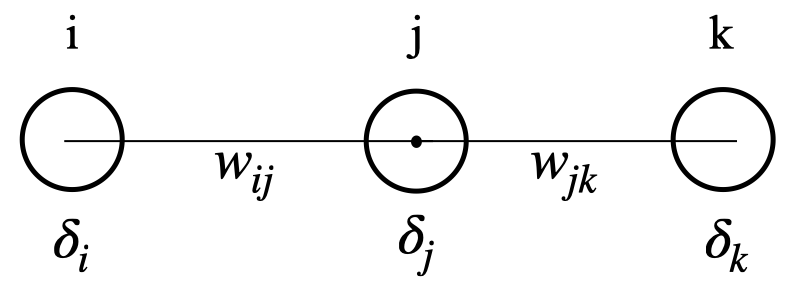
\includegraphics[scale=0.3]{Figs/1layer_nn}
\caption{A simple neural network consisting of one input neuron, one hidden layer neuron and one output neuron.}
\label{1layer_nn}
\end{center}
\end{figure}
This network makes the equations above simplify drastically.  To begin, the forward pass gives us that
\begin{equation}
a_i=f(z_i+b_i),
\end{equation}
\begin{equation}
z_j=w_{ij}a_i,
\end{equation}
\begin{equation}
a_j=f(z_j+b_j),
\end{equation}
and
\begin{equation}
z_k=w_{jk}a_j.
\end{equation}
Lastly,
\begin{equation}
a_k=f(z_k+b_k).
\end{equation}
We could combine all of this to get
\begin{equation}
a_k=f(w_{jk}f(w_{ij}f(z_i+b_i))),
\end{equation}
which clearly hows how the input to the network $z_i$ drives the output $a_k$ through the weights, biases and the activation function.

\begin{equation}
\delta_k=f'(z_k)(a_k-y_k),
\end{equation}
remembering that $a_k$ is the activation that comes out of the output neuron, and $y_k$ is what we want this neuron to produce. Additionally, 
\begin{equation}
\delta_j=f'(z_j)\delta_k w_{jk}.
\end{equation}
From these, the weight corrections can be found from $\Delta w_{right-layer\rightarrow left-layer}=\eta(\delta_{left-layer})(a_{right-layer})$ or
\begin{equation}
\Delta w_{jk}=\eta\delta_ka_j
\end{equation}
and
\begin{equation}
\Delta w_{ij}=\eta\delta_ja_i.
\end{equation}



\section{Build an optimized neural network model using matrices}

The codebase above works, which means it can be trained on vector pairs, and the loss function (target - output) summed across all output neurons will get arbitrarily small.  The code is slow though. Looking at the pseudo-code, you'll see at least one place where there are three nested loops.  Typically educational code like this won't be fast.

It turns out that it's better to approach modeling neural networks using matrices from linear algebra to handle all of the numbers. This falls under the purview of linear algebra, for which one should use a professional library's built-in matrix manipulation routines (matrix multiplication, dot product, etc.) wherever possible. In this work, Python and Numpy will be used for this, as shown here.  Below it will be shown how both the forward and backward passes can be (re)implemented with matrices.

\subsection{Forward pass}

Analyzing the forward pass will set the idea for using matrices.  Consider Equation~\ref{eqn_zy}, which is stated again here for clarity

\begin{equation}
z_{y}=\sum_x w_{xy} a_x + b_y
\end{equation}
which the input to neuron $y$ as fed from layer $x$. Let's write out a few terms of this sum for a few values of $y$. For $y=0$ we get

\begin{equation}
z_0=w_{00} a_0 + w_{10}a_1 + w_{20}a_2 + b_0,
\label{eqn_z0}
\end{equation}
$y=1$ gives
\begin{equation}
z_1=w_{01} a_0 + w_{11}a_1 + w_{21}a_2 + b_1,
\label{eqn_z1}
\end{equation}
and $y=2$
\begin{equation}
z_2=w_{02} a_0 + w_{12}a_1 + w_{22}a_2 + b_2.
\label{eqn_z2}
\end{equation}
Looking at it, the $z$'s can all be organized into a column vector like this

\begin{align}
     \begin{pmatrix}
           z_{0} \\
           z_{1} \\
           z_{2} \\
         \end{pmatrix}.
  \end{align}
  The weights can be contained in a matrix, like this
  
  \begin{align}
    \begin{pmatrix}
           w_{00} &w_{10} & w_{20}  \\
           w_{01} &w_{11} & w_{21}  \\
  	  w_{02} &w_{12} & w_{22} \\
         \end{pmatrix},
  \end{align}
  the $a$'s in another column vector like this
  \begin{align}
    \begin{pmatrix}
           a_{0} \\
           a_{1} \\
           a_{2} \\
         \end{pmatrix},
  \end{align}
  and finally, the $b$'s like this
    \begin{align}
    \begin{pmatrix}
           b_{0} \\
           b_{1} \\
           b_{2} \\
         \end{pmatrix}.
  \end{align}
Thus, Equations~\ref{eqn_z0}-\ref{eqn_z2} can be written as

  \begin{align}
    \begin{pmatrix}
           z_{0} \\
           z_{1} \\
           z_{2} \\
         \end{pmatrix}
=
 \begin{pmatrix}
           w_{00} &w_{10} & w_{20}  \\
           w_{01} &w_{11} & w_{21}  \\
  	  w_{02} &w_{12} & w_{22} \\
         \end{pmatrix}
     \begin{pmatrix}
           a_{0} \\
           a_{1} \\
           a_{2} \\
         \end{pmatrix}
+
    \begin{pmatrix}
           b_{0} \\
           b_{1} \\
           b_{2} \\
         \end{pmatrix}.
  \end{align}
This is a matrix equation that shows how the activations of the neurons in one layer $(a_0, a_1, a_2)$ feed the inputs of the neurons in the next layer $(z_0, z_1, z_2)$, via the interconnecting weights (the $w$'s), including the direct and additive effect of the biases on each neuron.  A single matrix multiplication between the weight matrix and activation vector, plus the biases will yield the inputs to the forward layer. This is contrasted with the two nested for-loops doing the same in the pseudo-code above.  Thus, our neural network might be thought of as that shown in Figure~\ref{nn_layers_weights}.

 \begin{figure}[h]
\begin{center}
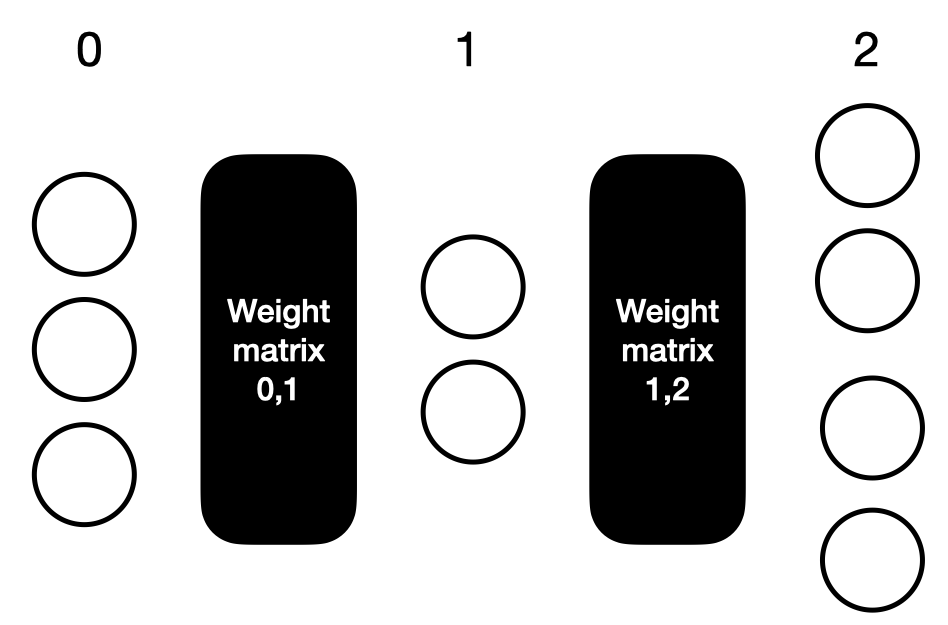
\includegraphics[scale=0.3]{Figs/nn_layers_weights}
\caption{A neural network with 3 input neurons, 2 neurons in the single hidden layer, and 4 neurons in the output layer.}
\label{nn_layers_weights}
\end{center}
\end{figure}

\subsubsection{Matrix sizes}

Here's another linear algebra consideration for our matrix-style network: the size (that is, the width and height, or rows and columns) of each weight matrix.  

As you can tell from the figure, the input layer has 3 neurons, which feed 2 neurons in the hidden layer, which in turn feed 4 neurons in the output layer. Thus, a goal of each weight matrix is to ``transform'' the activation vector of one layer (an $a$-vector), into the input of the next layer (the $z$-vector). In the case of the input to hidden layer here, a $3$ row $a$-vector from the input layer needs to be transformed into a $2$ row $z$-vector for the hidden layer.  Then the $2$ row $a$-vector of the hidden layer needs to be transformed into a $4$ row $z$-vector for the output layer. Here's how it might look for the input to hidden layer transformation

 \begin{align}
    \begin{pmatrix}
           z_{0} \\
           z_{1} \\
         \end{pmatrix}
=
   \begin{pmatrix}
           w_{00} &w_{10} & w_{20}  \\
           w_{01} &w_{11} & w_{21}  \\
         \end{pmatrix}
     \begin{pmatrix}
           a_{0} \\
           a_{1} \\
           a_{2} \\
         \end{pmatrix}
+
    \begin{pmatrix}
           b_{0} \\
           b_{1} \\
         \end{pmatrix}.
  \end{align}
Here you can see the $3$-row $a$ vector of the input layer being transformed into the $2$ row $z$ vector of the hidden layer. This is done with the $3$ column, $2$ row weight matrix.  

As matrix multiplication goes, the weight matrix between two layers must have the same number of columns as neurons in the activation (or source) layer, and the same number of rows as neurons in the destination layer.  This will handle any ``reshaping'' needed of the $a$-vectors from one layer getting properly shaped into $z$-vectors for the next layer.

Thus, in Figure~\ref{nn_reshape}, we see the $2$-row, $3$-column weight vector reshaping the $3$ neuron input vector into a $2$ neuron hidden layer vector. Then, a $4$-row, $2$-column weight vector reshapes the $2$ neuron hidden layer into a $4$ neuron output layer.

So,  the forward pass of a neural network is a series of matrix multiplications, that transform the input vector into the output vector, with potentially many multiplications in between. Each weight matrix scales a vector with the its numbers, and reshapes it with its size as needed by the next layer. So all we'll need to run a forward pass is a good matrix multiplication routine, not any clunky nested for-loops.


\subsubsection{Pseudo-code}

Here is pseudo-code that will take a vector {\tt input} and propagate it through the network.

\begin{lstlisting}[language=Python,
		basicstyle=\small\ttfamily,
                 numbers=left,
                 stepnumber=1,
                 numbersep=8pt,
                 tabsize=2,
                 showspaces=false,
                 breaklines=true,
                 showstringspaces=false,
                 columns=fullflexible]
function forward(input)
  layer_count = count of layers in network (input + hidden layers + output)
    
  #load up the input layer
  
  #input and bias are both vectors
  z = input + bias (input layer)
  
  #f is vectorized, meaning it'll operate on all elements of vector z
  a = f(z)
    
  #load up the rest of the network
  for layer = 0 to layer_count-1
    # dot is a professional matrix library function that 
    # will multiply a weight matrix by an activation vector
    # in Numpy it's called "dot."
    z = dot(weight matrix for layer to layer+1,a (layer)) + bias (layer+1)
    a = f(z)
  end
  #return the last activation, which will be that for the output layer
  return a
\end{lstlisting}


 \begin{figure}[h]
\begin{center}
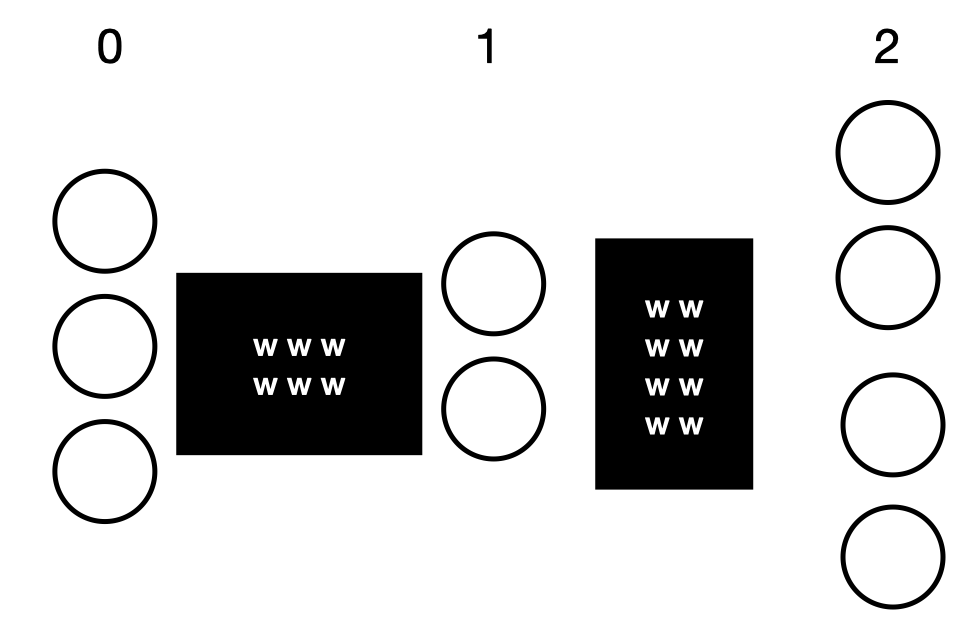
\includegraphics[scale=0.3]{Figs/nn_reshape}
\caption{Showing how the weight matrices must vary in size to reshape a source $a$-vector into the destination $z$-vector of the next layer.}
\label{nn_reshape}
\end{center}
\end{figure}

\subsection{Back propagation (the backward pass)}

The first consideration for a backward pass is in knowing two things for all neurons in the network, which are 1) the inputs to each (the $z$'s), and the error each neuron is introducing into the overall loss function of the network, which are the $\delta$ parameters.

\subsubsection{The z-vectors}

For later use in the error correcting (i.e. backward) pass, the $z$-values for all neurons must be captured and stored in as the forward pass progresses~\cite{karpathy,pytorch_history_tracking}.   This is not shown in the pseudo-code above, but essentially after each {\tt z=dot(...)} line, the matrix multiplication will return the $z$-values (or collectively $z$-vector) for that layer. These vectors must be stored with each iteration of the {\tt layer} forward pass, so they'll be available for later.  (In this work, each $z$-vector is appended to a Python list.)

\subsubsection{The $\delta$-vectors}
Next is the contribution of each neuron to the overall loss of the network. These are the $\delta$ parameters. Here, we will call a given error $\delta_k$. In our simplified notation, this mean $\delta$ of the $k$th neuron in later $k$.

\vspace{0.1in}
\subsubsection*{For the output layer}

The $\delta$'s for the output layer are straightforward to compute, since the desired target for each output neuron is known. (They are sometimes called the ``boundary condition'' for the network.) The formula is 

\begin{equation}
\delta_k=f'(z_k)(a_k-y_k),
\end{equation}

where $k$ is the $k$th neuron in the output layer, $f'(z_k)$ is the derivative of the activation function evaluated at $z_k$, $a_k$ is the activation (i.e. output) of the $k$th neuron in the output layer, and $y_k$ is the target value for the $k$th neuron in the output layer.  Thus, a $\delta$-vector can be compiled for the output layer, which will resemble (here show for $4$ neurons)

 \begin{align}
    \begin{pmatrix}
        \delta_0 \\
        \delta_1 \\
        \delta_2 \\
        \delta_3 \\
         \end{pmatrix}_k
 =
    \begin{pmatrix}
        f'(z_0)(a_0-y_0) \\
        f'(z_1)(a_1-y_1) \\
        f'(z_2)(a_2-y_2) \\
        f'(z_3)(a_3-y_3) \\
         \end{pmatrix},
 \end{align}
 where the subscript $k$ denotes the output layer of the network. We may also write this as
 
 \begin{align}
 {\vec \delta}_{\textrm{output layer}}=
    \begin{pmatrix}
        f'(z_0)(a_0-y_0) \\
        f'(z_1)(a_1-y_1) \\
        f'(z_2)(a_2-y_2) \\
        f'(z_3)(a_3-y_3) \\
        \vdots\\
         \end{pmatrix},
 \end{align}

 
 
\subsubsection*{For the hidden layers}

The $\delta$ parameters for the hidden layers are more complicated to compute, since the target values for such neurons are not known. They are, however, related to the target values of the network as a whole.  The $\delta$ value for a hidden layer is given by

\begin{equation}
\delta_j=f'(z_j)\sum_k\delta_k w_{jk}.
\label{eqn_dj}
\end{equation}
This equation will hold in general (meaning for any two adjacent layers in a network), but for the sake of instruction, let's consider the case of wanting to compute the $\delta$-vector for the first hidden layer that directly feeds the output layer. This will mean that $k$ denotes the output layer and $j$ the first hidden layer. 

Looking closely at the sum, one can see that finding a $\delta_j$ for a hidden layer neuron consists of propagating the known values of $\delta_k$ from the output layer, through all weights that connect them to a given neuron $j$ in the first hidden layer. This is what the sum does. The final step will be to evaluate the derivative of the activation function of the target neuron, at it's output level $z_j$. Let's look more closely.

Writing out a few terms of the sum (recalling that $k$ refers to a neuron in the output layer), we get
\begin{equation}
\sum_k\delta_k w_{jk}=\delta_0 w_{j0} + \delta_1 w_{j1} + \delta_2 w_{j2}+ \delta_3 w_{j3}\dots.
\end{equation}
Next, recall that $j$ refers to a neuron in the hidden layer. The first neuron will have $j=0$, then $j=1$, etc. So let's look at few more sequences here. For $j=0$ we get
\begin{equation}
\sum_k\delta_k w_{0k}=\delta_0 w_{00} + \delta_1 w_{01} + \delta_2 w_{02}+ \delta_3 w_{03}\dots.
\end{equation}
For $j=1$ we get
\begin{equation}
\sum_k\delta_k w_{1k}=\delta_0 w_{10} + \delta_1 w_{11} + \delta_2 w_{12}+ \delta_3 w_{13}\dots.
\end{equation}
These patterns reveal the operation needed to compute the sum: the sum is the {\sl dot product} between the $\delta$-vector of the output layer and the weight vector that connects the output layer to neuron $j$ (in the hidden layer). This is illustrated in Figure~\ref{nn_delta_connect}.

Intuitively, in order to compute $\delta_0$ in the hidden layer, we need all of the $\delta$ values in the output layer to ``feed'' their size through each's interconnecting weight to neuron $0$ in the hidden layer. This portion of the formula is $\delta_{0,\textrm{hidden layer}}\sim \delta_0 w_{00} + \delta_1 w_{01} + \delta_2 w_{02}+ \delta_3 w_{03}$.


 \begin{figure}[h]
\begin{center}
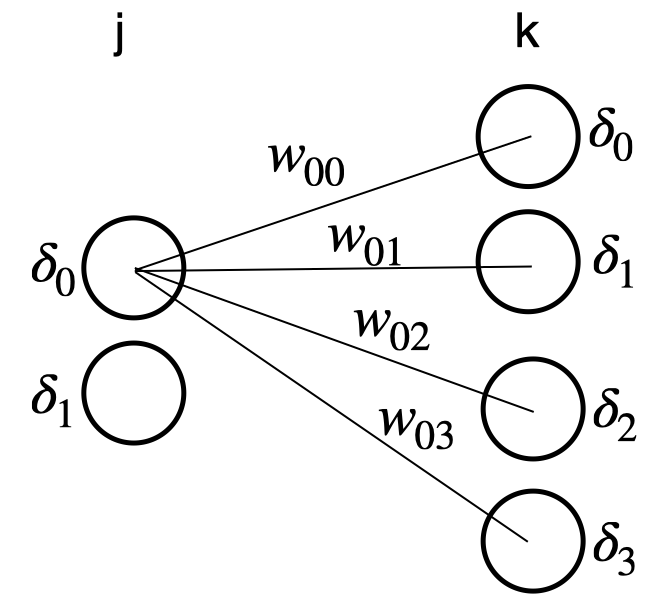
\includegraphics[scale=0.3]{Figs/nn_delta_connect}
\caption{Showing how $\delta$ for a neuron in the hidden layer is computed: the $\delta$-values of the \emph{output layer} are fed backwards into a given neuron in the \emph{hidden layer}, through the weights leading into the hidden layer neuron.  Here $\delta_{0,\textrm{hidden layer}}\sim \delta_0 w_{00} + \delta_1 w_{01} + \delta_2 w_{02}+ \delta_3 w_{03}.$}
\label{nn_delta_connect}
\end{center}
\end{figure}

This can all be computed from two things we already have, 1) the weight matrix connecting the two layers, and 2) the $\delta$ values from the output layer. Let's look first at the weight matrix connecting the two layers, which is (shaped properly to go from a $2$ neuron hidden layer, to a $4$ neuron output layer)
\begin{align}
 \begin{pmatrix}
           w_{00} &w_{10}  \\
           w_{01} &w_{11}  \\
  	  w_{02} &w_{12} \\
	   w_{03} &w_{13} \\
         \end{pmatrix}.
 \end{align}
 Notice the weights we need are in the first column, $w_{00}, w_{01}$, $w_{02}$, and $w_{03}$.  We also have the just-computed $\delta$-vector for the output layer, which was
 
 \begin{align}
    \begin{pmatrix}
        \delta_0 \\
        \delta_1 \\
        \delta_2 \\
        \delta_3 \\
         \end{pmatrix}_{k.}
  \end{align}
 So, the sum in Equation~\ref{eqn_dj} can be computed via a \emph{dot product} between the first column of the weight matrix and the $\delta$-vector for the output layer. The full result will be
 \begin{equation}
 \delta_0=f'(z_0){\vec w_{\textrm{0th col}}}\cdot{\vec \delta_{\textrm{output layer}}}.
 \end{equation}
 The $\delta$ values for the other neurons will come similarly as in
 \begin{equation}
 \delta_1=f'(z_1){\vec w_{\textrm{1st col}}}\cdot{\vec \delta_{\textrm{output layer}}},
 \end{equation}
  \begin{equation}
 \delta_2=f'(z_2){\vec w_{\textrm{2nd col}}}\cdot{\vec \delta_{\textrm{output layer}}},
 \end{equation}
 and
  \begin{equation}
 \delta_3=f'(z_3){\vec w_{\textrm{3rd col}}}\cdot{\vec \delta_{\textrm{output layer}}}.
 \end{equation}
 Hopefully you see how the $\delta$-vector for the first hidden layer can be constructed and that there is a pattern to the $\delta$-calculating pattern: for the $j$th neuron in a hidden layer, multiply the derivative of the $j$th neuron's activation function (evaluated at it's output $z_j$), by the dot product between the $j$th column of the weight matrix and the $\delta$-vector of the forward layer. 
 
 As far as matrix shapes go, the number of rows in the weight matrix will always match that of the length of the $\delta$-vector, since the number of rows in the weight matrix is what transforms the forward-going input vector into the number of eventual output neurons. (So, the dot product will always be evaluatable.)

 
The reason for pushing for mathematical conciseness (as in using a dot product) is that once again (for speed), the dot product function will come from a professional matrix library like NumPy.


As you might guess, there is a pattern for computing and using $\delta$-values. Once they are known for a given layer,  they are used in a similar manner to compute the $\delta$-values for the next (hidden layer) to the left of it, etc., all the way down to the input layer.
 
 \subsubsection{Correcting the weights}
 
Let's now look at how these $\delta$-vectors are used to correct the weights in a weight matrix. For orientation, let's assume we want to correct the weights in a given weight matrix, and know the $\delta$-vector for the layer to the right of the weight matrix (or the layer that the weight matrix feeds into during a forward pass).  So for example, suppose we want to correct the $w_{jk}$ weights and know the $\delta$-vector for layer $k$. The individual weights in the matrix need to be corrected, in order to nudge the all of the output neurons of the network to within some small distance of the desired target values of the network. 

The weight correction formula is
 
 \begin{equation}
 \Delta w_{jk}=-\eta\delta_k a_j,
 \end{equation}
 where we again focus on the weight matrix between the last hidden layer $j$ and the output layer $k$. Here, $\eta$ is a hyperparameter of the network, called the ``learning rate,'' and two more items are needed:
 \begin{enumerate}
 \item $a_j$, which is the activation of the hidden layer. This was found during the forward pass.  As mentioned in the forward pass discussion above, we need to store the $z$-vectors for each layer during the forward pass (the $z_j$ values).  The activation can be found from these since $a_j=f(z_j$), where $f$ is the activation function.
 
 \item $\delta_k$, which is the $\delta$ of the $k$th neuron in the output layer (its in $\delta$-vector of the output layer).
 \end{enumerate}
 
 Ideally, we'd like to once again exploit the speed of a matrix library, and avoid using any for-loops to do all of the weight corrections.  Our goal then is to construct a $\Delta w$ \emph{matrix}, that we can have the library add to the weight matrix, to nudge the weight values. In other words, if we have a weight matrix like this
 
 \begin{align}
 \begin{pmatrix}
           w_{00} &w_{10}  \\
           w_{01} &w_{11}  \\
  	  w_{02} &w_{12} \\
	   w_{03} &w_{13} \\
         \end{pmatrix},
 \end{align}
 we'd like to construct
 \begin{align}
 \begin{pmatrix}
           \Delta w_{00} & \Delta w_{10}  \\
           \Delta w_{01} & \Delta w_{11}  \\
  	  \Delta w_{02} & \Delta w_{12} \\
	  \Delta w_{03} & \Delta w_{13} \\
         \end{pmatrix},
 \end{align}
 and then have the library do an operation like
 \begin{align}
 \begin{pmatrix}
           w_{00} &w_{10}  \\
           w_{01} &w_{11}  \\
  	  w_{02} &w_{12} \\
	   w_{03} &w_{13} \\
         \end{pmatrix}
 +
 \begin{pmatrix}
           \Delta w_{00} & \Delta w_{10}  \\
           \Delta w_{01} & \Delta w_{11}  \\
  	  \Delta w_{02} & \Delta w_{12} \\
	  \Delta w_{03} & \Delta w_{13} \\
         \end{pmatrix},
 \end{align}
to correct the weights. Since we know a weight's correction is $\Delta w_{jk}=-\eta\delta_k a_j$, the $\Delta w$ matrix can be constructed by indexing through values of $j$ and $k$ (here $j$ is the column and $k$ is the row).


\vspace{0.1in}
\noindent\fbox{%
    \parbox{\textwidth}{%
       Note: In Section~\ref{definitions}, in the description of $w_{xy}$, we noted that the $w_{from-layer\rightarrow to-layer}$ notation might not have been the best choice, despite its natural fit in this work when referring to the weights between layers. Here is the reason why: in the standard notation of matrix algebra, when one writes something like $w_{jk}$, the row always comes first, then the column. So in this notation $j$ should be the row and $k$ the column.  This isn't the case in this work. So for example in the matrix above, where you see the element $w_{01}$, that should read $w_{10}$ since it's on row $1$, column $0$.
    }%
}
\vspace{0.1in}

\begin{align}
 \begin{pmatrix}
           \delta_0 a_0 & \delta_0 a_1  & \delta_0 a_2\\
           \delta_1 a_0 & \delta_1 a_1  & \delta_1 a_2\\
           \delta_2 a_0 & \delta_2 a_1 & \delta_2 a_2\\
         \end{pmatrix}.
         \label{da_matrix}
 \end{align}
You can see the $\delta$ values are ordered vertically in each column, and the $a$ values are ordered horizontally in each row~\cite{karpathy_youtube_01}. As tempting as it may seem with this matrix, there's no dot product to be taken here. Rather it's just a matrix construction we need to do, again while trying to avoid using any of our own for-loops.  We'll have a matrix library make two matrices, one that looks like this
 
 \begin{align}
 \begin{pmatrix}
           \delta_0 & \delta_0 & \delta_0\\
           \delta_1 & \delta_1 & \delta_1\\
           \delta_2 & \delta_2 & \delta_2\\
         \end{pmatrix},
 \end{align}
 and the other like this
 \begin{align}
 \begin{pmatrix}
           a_0 & a_1  & a_2\\
           a_0 & a_1  & a_2\\
           a_0 & a_1 & a_2\\
         \end{pmatrix}.
         \label{act_matrix}
 \end{align}
Then, the matrix library construct a third matrix which is the element-by-element product of the two matrices, which will result in the matrix of Equation~\ref{da_matrix} above.
 
 


\subsubsection*{Numpy}

Numpy allows for manipulation and creation of the matrices as discussed above. First, the function {\tt np.broadcast$\_$to} will take the activation vector (i.e. $(a_0,a_1,a_2,a_3)$) and ``broadcast it'' into a new shape.  Here, we'd like to shape the activation vector into a matrix that has a number of rows equal to the number of neurons in the forward layer, and columns equal to the length of the activation vector itself. 

As an example, if an activation vector is \verb|as_vector=[0.5, 0.2, 0.3, 0.1]|, then 
\begin{verbatim}
np.broadcast_to(as_vector,(5,len(as_vector)))
\end{verbatim}
will result in

\begin{verbatim}
[[0.5 0.2 0.3 0.1]
 [0.5 0.2 0.3 0.1]
 [0.5 0.2 0.3 0.1]
 [0.5 0.2 0.3 0.1]
 [0.5 0.2 0.3 0.1]].
 \end{verbatim}
 In other words, $5$ rows of the activation vector.  So we can make a matrix out of the activation vector by doing
 \begin{verbatim}
 mat_activations = np.broadcast_to(as_vector,(len(deltas[ahead]),len(as_vector)))
 \end{verbatim}
Here \verb|len(deltas[ahead])| is the number of neurons (and $\delta$ values) in the forward layer.  This will create \verb|mat_activations| as a matrix with the activation values all lined up in the rows of a matrix, as in Equation~\ref{act_matrix}.
 
 The delta values are handled similarly.  First, we take our $\delta$-vector and reshape it into a column array using 
 
 \begin{verbatim}
 ds_vector = deltas[ahead].reshape((len(deltas[ahead]),1))
 \end{verbatim}
 Next, this is broadcast into a matrix using
 \begin{verbatim}
 mat_deltas = np.broadcast_to(ds_vector,(len(deltas[ahead]),len(as_vector)))
 \end{verbatim} 
 The \verb|len(as_vector)| is used to ensure the $\delta$ matrix has as many columns as the activity matrix.  For example, if our delta vector was {\tt delta = np.array([1,2,3,4])}, then {\tt delta = np.reshape(delta,(len(delta),1))} would give
 
 \begin{verbatim}
 [[1]
 [ 2]
 [ 3]
 [ 4]]
 \end{verbatim}
 with the \verb|np.broadcast_to| line making this into
 \begin{verbatim}
      [[1, 1, 1, 1],
       [2, 2, 2, 2],
       [3, 3, 3, 3],
       [4, 4, 4, 4]]
 \end{verbatim}
 as needed.  With the activation values in rows, and the $\delta$ values in columns, the $\Delta w$ matrix can be found from \verb|np.multiply(mat_activations,mat_deltas)|. So, we've constructed the needed $\Delta w$ matrix using only the fast routines in the matrix library, and without any of our own for-loops. 
 

 
 
 









 


\section{Derivation of all back-propagation formulas}

The total loss of the network, $L_T$ is defined as

\begin{equation}
L_T=\frac{1}{2}\sum_n=(a_n - y_n)^2,
\label{loss}
\end{equation}
where the $n$ is summed over the $k$ neurons in the output layer.  It would have been more natural just to use $k$ instead of $n$ for in Equation~\ref{loss}, but this can lead to confusion later on (which we will note), in deriving the equations for backpropagation.

\subsection{Correcting weights feeding the output layer}

We begin with a left-to-right look at the network's architecture.  To begin we'll look at how the weights to the left of the output layer would need to be adjusted to nudge all $a_k$ values closer to their corresponding $y_k$ values.  For this, we'd like to know how the $w_{jk}$ weights affect $L_T$ or

\begin{equation}
\frac{\partial L_T}{\partial w_{jk}},
\end{equation}
where $w_{jk}$ are the weights connecting neurons in the leftward layer $j$ to neurons in the rightward layer $k$. Recall that the output layer is special, since its required outputs in the values of $y_n$ are known. Proceeding, we get that

\begin{equation}
\frac{\partial L_T}{\partial w_{jk}} = \sum_n (a_n-y_n)\frac{\partial a_n}{\partial w_{jk}}.
\label{jk_deriv}
\end{equation}

\noindent Finding $\partial a_n/\partial w_{jk}$ requires some careful consideration, and is related to our choosing of $n$ for the index to the sum (i.e. not $k$).  Here $n$ will run over all neurons in the output layer $k$, while $j$ refers to a specific neuron in the preceding layer and $k$ a specific neuron in the output layer.  

Upon careful inspection, we see that there is only one neuron in the output layer that has an activation with an explicit dependence on $w_{jk}$: is it the $a_n$ neuron when $n=k$, or neuron $a_k$. With this single neuron depending $w_{jk}$, only one term in the sum will be non-zero since $\partial a_n/\partial w_{jk}=0$ for all $n\ne k$. All $a_n$ terms with $n\ne k$ do not have any dependence on $w_{jk}$, so will all have derivatives with respect to $w_{jk}$ of zero. Thus, Equation~\ref{jk_deriv} becomes

\begin{equation}
\frac{\partial L_T}{\partial w_{jk}} = (a_k-y_k)\frac{\partial a_k}{\partial w_{jk}}.
\label{jk_deriv1}
\end{equation}
Finding $\partial a_k/\partial w_{jk}$ is fairly straightforward since $a_k=f(z_k)$ and $z_k=\sum_n w_{nk} a_n+b_k$, so
\begin{equation}
\frac{\partial a_k}{\partial w_{jk}} = \frac{\partial a_k}{\partial z_k}\frac{\partial z_k}{\partial w_{jk}}.
\end{equation}
First, we work on $\partial a_k/\partial z_k$, again noting tht $a_k=f(z_k$), with $f(x)$ the activation function in use. In general $f$ will be a function of one variable, like $x$, so $f=f(x)$. For the sigmoid function as an example, $f(x)=1/(1+e^{-x})$. For ReLU, $f(x)=\textrm{max}(0,x)$. So, $f'(z_k)$ means to differentiate the activation function with respect to $x$ and then evaluate the derivative at $x=z_k$. Since $a_k=f(z_k)$ we get

\begin{equation}
\frac{\partial a_k}{\partial z_k} = \left . \frac{\partial f}{\partial x} \right\vert_{x=z_k} = f'(z_k)
\end{equation}
Next,

\begin{equation}
\frac{\partial z_k}{\partial w_{jk}} = \frac{\partial}{\partial w_{jk}} \sum_n w_{nk} a_n + b_k.
\end{equation} 
which becomes
\begin{equation}
\frac{\partial z_k}{\partial w_{jk}} = \sum_n \frac{\partial w_{nk}}{\partial w_{jk}} a_n + w_{nk} \frac{\partial a_n}{\partial w_{jk}}+ \frac{\partial b_k}{\partial w_{jk}}.
\label{dz_k_wjk}
\end{equation} 
Here we must examine all three terms in the sum, remembering that $n$ is summing over the $j$ neurons. First the term that has a $w_{jk}$ in it to differentiate 

\begin{itemize}
\item First term: All derivatives of $w_{nk}$ with respect to $w_{jk}$ are zero unless $n=j$, so all of these terms will be zero except for $\partial{ w_{jk}}/\partial{w_{jk}}$ which is $1$. So this term becomes $a_j$.  Weights are independent parameters, and one will not depend on another, hence all of the zero derivatives (unless the weight is differentiated with respect to itself).

\item Second term: No activation $a_n$ in the $j$ layer will depend on a weight $w_{jk}$, since the $a_j$ neurons all feed into the $w_{jk}$ weights.  So this term is zero for all $n$.

\item Third term:  No bias depends on any weight so this term is zero.

\end{itemize} 
Thus Equation~\ref{dz_k_wjk} becomes
\begin{equation}
\frac{\partial z_k}{\partial w_{jk}} = a_j.
\end{equation} 
Collecting these results, we arrive at

\begin{equation}
\frac{\partial L_T}{\partial w_{jk}} = (a_k-y_k) f'(z_k) a_j.
\label{jk_deriv1}
\end{equation}
This is our first equation for back-propagation and we note it's left-to-right nature: It tells us how any changing any weight to the left of the output layer, $w_{jk}$ will affect $L_T$, which is computed from the rightward (more forward) output layer.

As per standard treatment of back-propagation, we can define $\delta_k$ to be

\begin{equation}
\delta_k = f'(z_k)(a_k-y_k),
\label{delta_k}
\end{equation}
so Equation~\ref{jk_deriv1} becomes

\begin{equation}
\frac{\partial L_T}{\partial w_{jk}} = \delta_k a_j,
\label{bp1}
\end{equation}
which is the same as Equation BP4 in Ref.\cite{nielson}.

One last reminder of the notation: the correction to weight $w_{jk}$, which is the weight connecting neuron $j$ (in layer $j$) to neuron $k$ (in layer $k$) is the $\delta_k$ of the $k$th neuron (in layer $k$) times the activation of neuron $a_j$ (in layer $j$). Thishas some intuitive meaning.  

The effect of a weight on the loss function or ${\partial L_T}/{\partial w_{jk}}$ is the error contributed by the forward layer $(\delta_k)$ times the strength of the neuron that feeds it $(a_j)$. So the weight-on-the-loss dependency is related to the ultimate error in the forward layer times the strength of the firing of the neuron that (partly) contributed to the error. Kind of makes sense on two fronts: 1) a small error will mean ${\partial L_T}/{\partial w_{jk}}$ is small, and why shouldn't it be? If the error is small, this part of the network's contribution to affecting the loss should. be small.  2) if the neuron firing is small, again its contribution to changing the loss should also be small.

\subsubsection{A short numerical example}

A tutorial on PyTorch~\cite{pytorch} has a nice example that shows the meaning of ${\partial L_T}/{\partial w_{jk}} = \delta_k a_j$, and how it works. Let's take a look at it, as it will illustrate the meaning of Equation~\ref{bp1}. You can find the original code at Ref.~\cite{pytorch_grad}.

\begin{lstlisting}[language=Python,
		basicstyle=\small\ttfamily,
                 numbers=left,
                 stepnumber=1,
                 numbersep=8pt,
                 tabsize=2,
                 showspaces=false,
                 breaklines=true,
                 showstringspaces=false,
                 columns=fullflexible]
import numpy as np
import math

x = np.linspace(-math.pi, math.pi, 2000)
y = np.sin(x)

a = np.random.randn()
b = np.random.randn()
c = np.random.randn()
d = np.random.randn()

learning_rate = 1e-6
for t in range(2000):
    y_pred = a + b * x + c * x ** 2 + d * x ** 3

    loss = np.square(y_pred - y).sum()

    # Backprop to compute gradients of a, b, c, d with respect to loss
    grad_y_pred = 2.0 * (y_pred - y)
    grad_a = grad_y_pred.sum()
    grad_b = (grad_y_pred * x).sum()
    grad_c = (grad_y_pred * x ** 2).sum()
    grad_d = (grad_y_pred * x ** 3).sum()

    # Update weights
    a -= learning_rate * grad_a
    b -= learning_rate * grad_b
    c -= learning_rate * grad_c
    d -= learning_rate * grad_d

print(f'Result: y = {a} + {b} x + {c} x^2 + {d} x^3')
\end{lstlisting}
The goal of this code is to use back propagation to estimate the coefficients of the polynomial $y=a+bx+cx^2+dx^3$ that would make it approximate $\sin(x)$.  The coefficients here are like the weights in a neural network.  Here's how the code works:

\begin{itemize}
\item The definitions of {\tt x} and {\tt y} set up $x$ and $y$ coordinate space as in $y(x)=\sin(x)$ for $-\pi\le x\le \pi$.

\item The lines for {\tt a=...}, {\tt b=...},  {\tt c=...} and {\tt d=...} initialize all of the coefficients in the polynomial to (normally distributed) random values.

\item Now, a ``back propagation loop'' is started.  The predicted $y$ is computed in {\tt y$\_$pred}, and the loss, which is a measure of how far off the prediction is versus the $\sin$ data (i.e. {\tt y}). The loss function is $L=\sum_n (y_{pred(n)}-y_n)^2$.

\item Now, the gradients are computed, which are the derivative of the loss function with respect to each coefficient, so the code will compute ${\partial L}/{\partial a}$, ${\partial L}/{\partial b}$, ${\partial L}/{\partial c}$, and ${\partial L}/{\partial d}$. Let's run through these.

\begin{enumerate}
\item ${\partial L}/{\partial a}$:

\begin{equation}
\frac{\partial L}{\partial a}=2 \sum_n (y_{pred}-y)\cdot \frac{\partial y_{pred}}{\partial a}.
\end{equation}
Now, ${\partial y_{pred}}/{\partial a}=1$, so ${\partial L}/{\partial a}=2\sum_n  (y_{pred}-y)$, which all goes into the assignment of \verb|grad_a| in the code.

\item ${\partial L}/{\partial b}$:
\begin{equation}
\frac{\partial L}{\partial b}=2 \sum_n (y_{pred}-y)\cdot \frac{\partial y_{pred}}{\partial b}.
\end{equation}
which is ${\partial L}/{\partial b}=2\sum_n  (y_{pred}-y)\cdot x$ (noting that ${\partial y_{pred}}/{\partial b}=x$).

\item The others follow similarly with  ${\partial L}/{\partial c}=2\sum_n  (y_{pred}-y)\cdot x^2$ and  ${\partial L}/{\partial d}=2\sum_n  (y_{pred}-y)\cdot x^3$.

\end{enumerate}
You can see all of these defined in the code for \verb|grad_a=...|, \verb|grad_b=...|, \verb|grad_c=...|, and \verb|grad_d=...|.

\item Lastly, all of the coefficients are updated using the general form that
\\
$\Delta$\verb|coeff=learning_rate|$\times$\verb|gradients|.  Note that the coefficient correction formulas all contain a product of two items: 1) a term reflecting the loss function's behavior and 2) the ``strength'' of the variable the weight is associated with.  Equation~\ref{bp1} has the same elements: $\delta_k$ is related to the loss function's behavior and $a_j$, related to the strength of the neuron firing into the weight.

\end{itemize}
When the code above is run, it arrives at $y(x) =  0.0237 +  0.8476 x + -0.004 x^2 -0.0920 x^3$, which is shown compared to  $\sin(x)$ in Figure~\ref{bp_sin}. The process did a pretty good job.


\begin{figure}[h]
\begin{center}
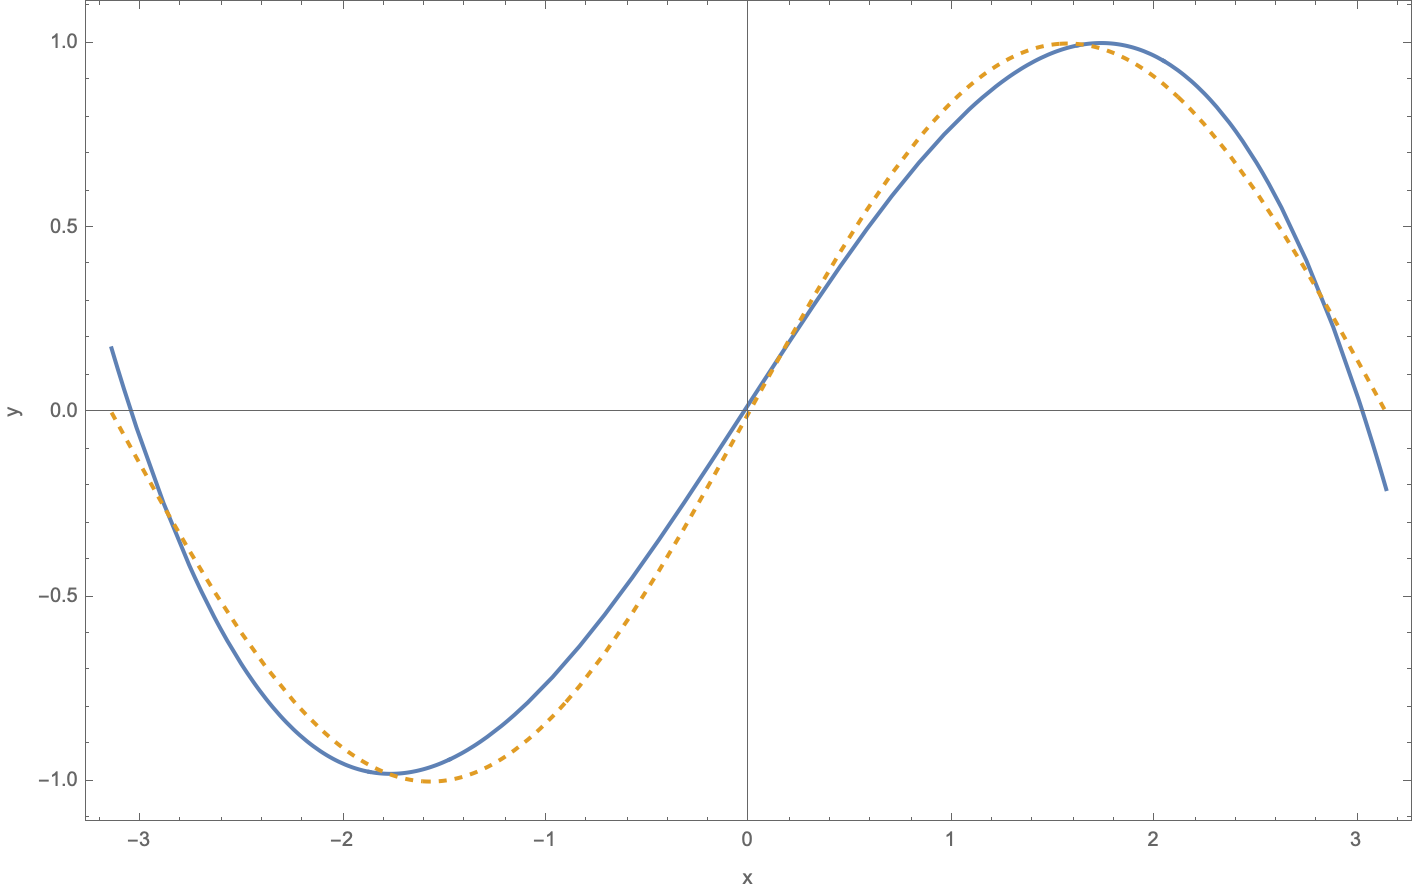
\includegraphics[scale=0.6]{Figs/bp_sin.png}
\caption{$\sin(x)$ (dotted) vs $y(x)$ (solid) approximated from the gradient descent code above.}
\label{bp_sin}
\end{center}
\end{figure}


\subsection{Correcting weights feeding a hidden layer}

The challenge with correcting the weights feeding a  hidden layer is that the target output of a hidden layer is not known.  Recall for an output layer, $y_n$ is known so the error for the output layer $a_n-y_n$ was available. Here we see how to correct the weights $w_{ij}$ for a hidden later, whose error is not known.

As above, we rely on only on calculus and begin by differentiating the loss function with respect to $w_{ij}$, which are weights feeding the hidden layer as in

\begin{equation}
\frac{\partial L_T}{\partial w_{ij}} = \sum_n (a_n-y_n)\frac{\partial a_n}{\partial w_{ij}}.
\label{ij_deriv}
\end{equation}

Recall that $a_n$ is an output layer neuron activation, and there is no explicit dependence of $a_n$ on $w_{ij}$, as these weights to not directly connect to any of the $a_n$ output neurons. We know there is an {\sl implicit dependence} though, owing to the hyperconnected nature of the neural network; certainly data flow through a hidden layer affects the output of the network.  

So, the derivative exists (and is not necessarily zero), but arriving at a proper  expression for its derivative will require some careful work. We will rely on the rules of calculus to carry us through.  Lastly, the $\sum_n$ persists at the moment, since we cannot state any conditions that make $\partial a_n/\partial w_{ij}=0$, as a function of $n$ (as we did in the previous section).

Proceeding, we know that $a_n=f(z_n)$ and $z_n=\sum_m w_{mn} a_m + b_n$, where $m$ is summed over the $j$ neurons in the first hidden-layer to the left of the output layer. We again need to use a neutral index like $m$ to avoid confusion with the $ij$ use in the derivative $\partial a_n/\partial w_{ij}$.  With this

\begin{equation}
a_n=f\left(\sum_m w_{mn} a_m + b_n\right),
\end{equation}

\noindent which shows the subtle dependence of $a_n$ on $w_{ij}$: $a_n$ clearly depends on $a_m$, and $a_m$ depends on the weights to the left of it, which are the $w_{ij}$ weights (again, $m$ is summed over the $j$ neurons). So, we see $a_n$ depends on $a_m$ and $a_m$ depends on $w_{ij}$, thus $a_n$ depends on $w_{ij}$ (just not with the explicit simplicity of $a_n$ on $w_{jk}$ as in the section above). Looking at Figure~\ref{nn}, you can see from the connectedness of the network that the output neurons $a_n$ would indeed depend on the $w_{ij}$ weights.

Since $a_n$ is a composite function of the activation function evaluated at $z_n$ as in $a_n=f(z_n)$, we apply the chain rule to get

\begin{equation}
\frac{\partial a_n}{\partial w_{ij}} = \frac{\partial a_n}{\partial z_n} \frac{\partial{z_n}}{\partial w_{ij}}.
\label{d_an_wij}
\end{equation}

\noindent Now, 

\begin{equation}
\frac{\partial{ a_n}}{\partial z_n}=\left . \frac{\partial f}{\partial x} \right\vert_{x=z_n}=f'(z_n)
\end{equation}

\noindent and using the product rule to allow subtle interdependencies between variables to be handled properly, 

\begin{equation}
\frac{\partial{z_n}}{\partial w_{ij}}=\sum_m \frac{\partial w_{mn}}{\partial w_{ij}} a_m + w_{mn}\frac{\partial a_m}{\partial w_{ij}} + \frac{\partial b_n}{\partial w_{ij}}.
\end{equation}
Two simplifications are seen. First, weights in different layers are all independent parameters, all $\partial w_{mn}/\partial w_{ij}=0$ ($w_{mn}\sim w_{jk}$).  Second, any bias is independent of any weight, so $\partial b_n/\partial w_{ij}=0$. Thus, the above reduces to

\begin{equation}
\frac{\partial{z_n}}{\partial w_{ij}}=\sum_m w_{mn}\frac{\partial a_m}{\partial w_{ij}}.
\end{equation}

\noindent Now, only term in the sum that has a non-zero derivative is when $m=j$, since of all of the $ij$ weights, the $j$th neuron ($a_j$) is the only one fed by the one weight $w_{ij}$.  Thus


\begin{equation}
\frac{\partial{z_n}}{\partial w_{ij}}=w_{jn}\frac{\partial a_j}{w_{ij}}.
\label{zn_by_wij}
\end{equation}

This puts us in a good position, since we're left with just $\partial a_j/\partial w_{ij}$.  We know that the $a_j$ neurons have an explicit dependence on $w_{ij}$, as these are the weights that feed the $a_j$ neurons directly, so the derivative must have an analytic answer.

As before, we know that $a_j=f(z_j)$ with $z_j=\sum_n w_{nj}a_n+b_j$ (with $n$ summed over the $i$ neurons)

\begin{equation}
\frac{\partial{a_j}}{\partial w_{ij}}=\frac{\partial{a_j}}{\partial z_j} \frac{\partial z_j}{\partial w_{ij}}
\label{aj_by_wij}
\end{equation}
and

\begin{equation}
\frac{\partial{a_j}}{\partial z_j}=\left . \frac{\partial f}{\partial x}\right\vert_{x=z_j}=f'(z_j).
\end{equation}
Lastly,

\begin{equation}
\frac{\partial z_j}{w_{ij}}=\sum_n \frac{\partial w_{nj}}{\partial w_{ij}}a_n+w_{nj}\frac{\partial a_n}{\partial w_{ij}}+\frac{\partial b_j}{\partial w_{ij}}.
\label{zj_by_wij}
\end{equation}
We know $\partial b_j/\partial w_{ij}$ is zero since no biases depend on any weights, but we are still left with two non-obvious derivatives, $\partial w_{nj}/\partial w_{ij}$ and $\partial {a_n}/{\partial w_{ij}}$.  

First, we see that $\partial w_{nj}/\partial w_{ij}=1$ if $n=i$ and $0$ otherwise, since two different weights are independent of one another.  

Second,  at $n=i$, $\partial {a_i}/{\partial w_{ij}}=0$ since the the activation of a neuron does not depend on the weights that it feeds forward into. So Equation~\ref{zj_by_wij} becomes

\begin{equation}
\frac{\partial z_j}{w_{ij}}=a_i.
\end{equation}
With these results, Equation~\ref{aj_by_wij} becomes

\begin{equation}
\frac{\partial{a_j}}{\partial w_{ij}}=f'(z_j)a_i,
\end{equation}
allowing Equation~\ref{zn_by_wij} to become

\begin{equation}
\frac{\partial z_n}{\partial w_{ij}}=w_{jn}f'(z_j)a_i,
\end{equation}
and Equation~\ref{d_an_wij}

\begin{equation}
\frac{\partial a_n}{\partial w_{ij}} =f'(z_n)w_{jn}f'(z_j)a_i.
\label{d_an_wij_filled}
\end{equation}
Plugging this into Equation~\ref{ij_deriv}, we get

\begin{equation}
\frac{\partial L_T}{\partial w_{ij}} = \sum_n (a_n-y_n)f'(z_n)w_{jn}f'(z_j)a_i.
\end{equation}
With possible confusion over the sum indices behind us, we can put $n\rightarrow k$ into this equation to get

\begin{equation}
\frac{\partial L_T}{\partial w_{ij}} = \sum_k (a_k-y_k)f'(z_k)w_{jk}f'(z_j)a_i.
\end{equation}
Using the definition of $\delta_k$ in Equation~\ref{delta_k} this becomes

\begin{equation}
\frac{\partial L_T}{\partial w_{ij}} = \sum_k \delta_k w_{jk}f'(z_j)a_i.
\end{equation}
Additionally, to see a form consistent with Equation~\ref{bp1}, we define $\delta_j$ as

\begin{equation}
\delta_j =  f'(z_j) \sum_k \delta_k w_{jk},
\end{equation}
so $\partial L_T/\partial w_{ij}$ becomes

\begin{equation}
\frac{\partial L_T}{\partial w_{ij}} = \delta_j a_i.
\end{equation}

 

\noindent This result agrees with the equation in Section 4.5 of Ref.~\cite{swarthmore}.


\subsubsection{One more time}

It appears that a pattern is emerging on the effect of weights on the network loss:  ${\partial L}/{\partial w_{xy}}=\delta_y a_x$.  Note again, $w_{xy}$ is the weight connecting neuron $x$ (in layer $x$) to neuron $y$ (in layer $y$), with $y$ always being the layer that $x$ feeds into (in the forward data-flow sense of the network).  The reversal of the indices across the equal sign means we need $\delta$ of the forward (or rightward) layer and the activation of the backward (or leftward) layer.

In Figure~\ref{nn}, we'll imagine one more layer $h$ to the left of layer $i$, and consider $\partial L/\partial w_{hi}$. Without going through the steps, which are all have similar considerations to the above, we arrived at

\begin{equation}
\frac{\partial L_T}{\partial w_{hi}}=\sum_k (a_k-y_k)f'(z_k)\sum_j w_{jk} f'(z_j) w_{ij} f'(z_i) a_h.
\end{equation}
Let's rearrange this some to get
\begin{equation}
\frac{\partial L_T}{\partial w_{hi}}=\sum_j w_{ij} f'(z_j)\sum_k (a_k-y_k)f'(z_k) w_{jk} f'(z_i) a_h.
\end{equation}
Remembering that $\delta_k=f'(z_k)(a_k-y_k)$ we get
\begin{equation}
\frac{\partial L_T}{\partial w_{hi}}=\sum_j w_{ij} f'(z_j)\sum_k\delta_k w_{jk} f'(z_i) a_h.
\end{equation}
Also using that $\delta_j=f'(z_j)\sum_k \delta_k w_{jk}$ we get
\begin{equation}
\frac{\partial L_T}{\partial w_{hi}}=\sum_j w_{ij} f'(z_i)\delta_j a_h.
\end{equation}
Doing some rearranging
\begin{equation}
\frac{\partial L_T}{\partial w_{hi}}=f'(z_i) \sum_j w_{ij}\delta_j a_h,
\end{equation}
we can now define
\begin{equation}
\delta_i=f'(z_i) \sum_j \delta_j w_{ij}
\end{equation}
for which we get
\begin{equation}
\frac{\partial L_T}{\partial w_{hi}}=\delta_i a_h
\label{dL_by_dwhi}
\end{equation}
Once again, we see a pattern like  ${\partial L_T}/{\partial w_{xy}}=\delta_ya_x$. This tell us the following about back-propagation:

\begin{itemize}
\item To correct the weights connecting two layers, with layer $x$ feeding layer $y$, you need $\delta_y$ from the forward layer and the activations from the backward $(x)$ layer.  

\item The $\delta_x$ parameters all depend on one another, all the way ``up'' to the original delta that comes from a direct comparison of the output of the network to the needed target for the applied input. 

\item An unknown $\delta_x$ (for neuron $x$ in layer $x$) that is a layer back from a known $\delta_{x+1}$ is found by propagating (summing) the known $\delta_{x+1}$ values backward through all weights connecting the known $\delta_{x+1}$ and unknown $\delta_x$ values. This will be multiplied by the derivative of the activation function evaluated at $z_x$ for backward neuron $x$ to arrive at the value for $\delta_x$.

\item  It appears that ${\partial L_T}/{\partial w_{xy}}=\delta_ya_x$ depends on the forward feed strength of a neuron (its activation, $a_x$) and the amount of error this caused in the forward layer it feeds ($\delta_y$).   To confirm the pattern, let's repeat the derivation one more time. 

\end{itemize}

\subsection{Correcting neuron biases}

Next, we examine how a the bias of a neuron affects the network loss.  Here we still define the total loss, $L_T$ as

\begin{equation}
L_T=\frac{1}{2}\sum_n (a_n-y_n)^2,
\end{equation}
and would like to know

\begin{equation}
\frac{\partial L_T}{b_n}=\sum (a_n-y_n)\frac{\partial a_n}{\partial b_n},
\end{equation}
to see how $b_n$ affects $L_T$. That is, how the bias of an output neuron, $b_n$ (for neuron $a_n$) affects $L_T$. The derivative here is ${\partial a_n/\partial b_n}$, which is

\begin{equation}
\frac{\partial a_n}{\partial b_n}=\frac{\partial a_n}{\partial z_n}\frac{\partial z_n}{\partial b_n}.
\end{equation}
Knowing that $z_n=\sum_j w_{jn}a_j+b_n$, we see that ${\partial z_n}/{\partial b_n}=1$ and as seen above ${\partial a_n}/{\partial z_n}=f'(z_n)$, thus

\begin{equation}
\frac{\partial L_T}{b_n}=\sum (a_n-y_n)f'(z_n).
\end{equation}
Now, allowing $n\rightarrow k$, we get

\begin{equation}
\frac{\partial L_T}{b_k}=\sum (a_k-y_k)f'(z_k),
\end{equation}
which is
\begin{equation}
\frac{\partial L_T}{b_k}=\delta_k,
\end{equation}
as defined in Equation~\ref{delta_k}. So it appears as if a bias alters the loss directly by the magnitude of $\delta$ of a neuron itself. 

\subsubsection{Another look}
Let's look one layer back to confirm this emerging pattern on how loss depends on $\delta$ of a neuron.

\begin{equation}
\frac{\partial L_T}{\partial b_j}=\sum_n (a_n-y_n)\frac{\partial a_n}{\partial b_j}.
\label{LT_by_bj}
\end{equation}
As before
\begin{equation}
\frac{\partial a_n}{\partial b_j}=\frac{\partial a_n}{\partial z_n}\frac{\partial z_n}{\partial b_j}.
\label{an_by_bj}
\end{equation}
We've seen that ${\partial a_n}/{\partial z_n}=f'(z_n)$. Next, knowing that $z_n=\sum_m w_{mn}a_m+b_n$, we write that
\begin{equation}
\frac{\partial z_n}{\partial b_j}=\sum_m\frac{\partial w_{mn}}{\partial b_j}a_m+w_{mn}\frac{\partial a_m}{\partial b_j}+\frac{\partial b_n}{\partial b_j}.
\end{equation}
Now, ${\partial b_n}/{\partial b_j}=0$ since no two neuron biases depend on one another. Also, ${\partial w_{mn}}/{\partial b_j}=0$ since no weight depends on any bias.  So we are left with
\begin{equation}
\frac{\partial z_n}{\partial b_j}=\sum_m w_{mn}\frac{\partial a_m}{\partial b_j}.
\end{equation}
Here we see that only $m=j$ has a non-zero ${\partial a_m}/{\partial b_j}$, since the activation of a neuron can only depend on its own bias. Thus, we get that 
\begin{equation}
\frac{\partial z_n}{\partial b_j}=w_{jn}\frac{\partial a_j}{\partial b_j}.
\end{equation}
Thus Equation~\ref{an_by_bj} can assembled to be
\begin{equation}
\frac{\partial a_n}{\partial b_j}=f'(z_n)w_{jn}\frac{\partial a_j}{\partial b_j}.
\end{equation}
And, using Equation~\ref{an_by_bj} with $n=j$, we get
\begin{equation}
\frac{\partial a_j}{\partial b_j}=\frac{\partial a_j}{\partial z_j}\frac{\partial z_j}{\partial b_j}.
\end{equation}
Here, ${\partial a_j}/{\partial z_j}=f'(z_j)$ and ${\partial z_j}/{\partial b_j}=1$
\begin{equation}
\frac{\partial a_j}{\partial b_j}=f'(z_j).
\end{equation}
Since $z_j=\sum_m w_{mj}a_m+b_j$ and since  $m$ is summed over the $i$ neurons, neither $w_{mj}$ or $a_m$ (or $a_i$) depend on $b_j$.
These can be put into Equation~\ref{an_by_bj} to get
\begin{equation}
\frac{\partial a_n}{\partial b_j}=f'(z_n)f'(z_j).
\label{an_by_bj1}
\end{equation}
Finally, Equation~\ref{LT_by_bj} now becomes
\begin{equation}
\frac{\partial L_T}{\partial b_j}=\sum_n (a_n-y_n)f'(z_n)f'(z_j).
\end{equation}
Letting $n\rightarrow k$, we get
\begin{equation}
\frac{\partial L_T}{\partial b_j}=\sum_k (a_k-y_k)f'(z_k)f'(z_j),
\end{equation}
which is 
\begin{equation}
\frac{\partial L_T}{\partial b_j}=f'(z_j)\sum_k (a_k-y_k)f'(z_k),
\end{equation}
or 
\begin{equation}
\frac{\partial L_T}{\partial b_j}=\delta_j.
\end{equation}
So indeed, the pattern holds: the dependence of the network loss on a neuron bias is the value of $\delta$ of that  neuron. 


\section{Physics Informed Neural Network (PINN)}

Idea: is it also possible to feed derivatives forward through a neural network.

Assume a three-layer neural network $i$, $j$, and $k$, with a single input neuron with input $z_1$. In physics, this will be a single variable of integration like $t$. As usual, this single input neuron is activated with $a_1=f(z_1)$, and this neuron is connected to the $j$th neuron in the forward layer via weight $w_{1j}$.  The next layer $j$ is found as

\begin{equation}
a_j=f\left(w_{1j} a_1\right),
\end{equation}
and the next as 
\begin{equation}
z_k=\sum_j w_{jk} a_j,
\end{equation}
with
\begin{equation}
a_k=f(z_k).
\end{equation}

\subsection{Working backward to find the derivative of the network}
\label{dforward}

Starting with the output of the network, We differentiate the output $a_k$ with respect to the input $z_1$:
\begin{equation}
\frac{da_k}{dz_1}=f'(z_k)\frac{dz_k}{dz_1}.
\end{equation}
But 
\begin{equation}
\frac{dz_k}{dz_1}=\sum_j w_{jk}\frac{da_j}{dz_1},
\end{equation}
with 
\begin{equation}
\frac{da_j}{dz_1}=f'(w_{1j}{a_1})w_{1j}\frac{da_1}{dz_1}.
\end{equation}
Lastly,
\begin{equation}
\frac{da_1}{dz_1}=f'(z_1),
\end{equation}
so
\begin{equation}
\frac{da_j}{dz_1}=f'(w_{1j}{a_1})w_{1j}f'(z_1).
\end{equation}
The final result is then
\begin{equation}
\frac{dz_k}{dz_1}=\sum_j w_{jk}f'(w_{1j}{a_1})w_{1j}f'(z_1).
\end{equation}
Rearranging and using $a_1=f(z_1)$we get
\begin{equation}
\frac{dz_k}{dz_1}=f'(z_1)\sum_j w_{1j}w_{jk}f'(w_{1j}{f(z_1)}).
\label{dbase}
\end{equation}
Using this expression as a base, we see that higher derivatives are possible with respect to the input variable $z_1$, as
\begin{equation}
\frac{d^2z_k}{dz_1^2}=f''(z_1)\sum_j w_{1j}w_{jk}f'(w_{1j}{f(z_1)}) + f'(z_1)\sum_j w_{1j}w_{jk}f''\left(w_{1j}f(z_1)\right)\frac{d(w_{1j}f(z_1))}{dz_1},
\end{equation}
which becomes
\begin{equation}
\frac{d^2z_k}{dz_1^2}=f''(z_1)\sum_j w_{1j}w_{jk}f'(w_{1j}{f(z_1)}) + f'(z_1)\sum_j w_{1j}w_{jk}f''\left(w_{1j}f(z_1)\right)w_{1j}f'(z_1).
\end{equation}

\subsection{Working forward to find the derivative of the network}
\label{dforward}

Let's find the derivative of the network by starting with the input. We know that 

\begin{equation}
z_j=w_{1j}{a_1},
\end{equation}
with the activation being
\begin{equation}
a_j=f(z_j),
\end{equation}
with
\begin{equation}
\label{dcore_idea}
\frac{da_j}{dz_1}=f'(w_{1j}a_1)w_{1j}\frac{da_1}{dz_1}.
\end{equation}
Now with
\begin{equation}
z_k=\sum_j w_{jk} a_j,
\end{equation}
we can write
\begin{equation}
\frac{dz_k}{dz_1}=\sum_j w_{jk}\frac{da_j}{dz_1},
\end{equation}
which becomes
\begin{equation}
\frac{dz_k}{dz_1}=\sum_j w_{jk}f'(w_{1j}a_1)w_{1j}\frac{da_1}{dz_1}.
\end{equation}
Now
\begin{equation}
\frac{da_1}{dz_1}=f'(z_1)
\end{equation}
so
\begin{equation}
\frac{dz_k}{dz_1}=\sum_j w_{jk}f'(w_{1j}a_1)w_{1j}f'(z_1),
\end{equation}
which when rearranging gives
\begin{equation}
\frac{dz_k}{dz_1}=f'(z_1)\sum_j w_{1j} w_{jk}f'(w_{1j}f(z_1)),
\end{equation}
which is the same as Eqn.~\ref{dbase}.

\subsection{Forward with a larger network}

Let's find the derivative of the network by starting with the input. For $i$ input neurons initialized each with $z_i$ then activated with $a_i=f(z_i)$ we know that 

\begin{equation}
z_j=\sum_i w_{ij}a_i,
\end{equation}
with
\begin{equation}
a_j=f(z_j),
\end{equation}
or
\begin{equation}
a_j=f\left(\sum_i w_{ij}a_i\right).
\end{equation}
Now,
\begin{equation}
\frac{da_j}{dz_1}=f'\left(\sum_i w_{ij}a_i\right)\left(\frac{d}{dz_1}\sum_i w_{ij}a_i\right),
\end{equation}
which is
\begin{equation}
\frac{da_j}{dz_1}=f'\left(\sum_i w_{ij}a_i\right)\left(\sum_i w_{ij}\frac{da_i}{dz_1}\right).
\end{equation}
But
\begin{equation}
\frac{da_i}{dz_i}=f'(z_i),
\end{equation}
so
\begin{equation}
\label{dcore1}
\frac{da_j}{dz_1}=f'\left(\sum_i w_{ij}a_i\right)\left(\sum_i w_{ij}f'(z_i)\right).
\end{equation}
Now with
\begin{equation}
z_k=\sum_j w_{jk} a_j,
\end{equation}
we can write
\begin{equation}
\frac{dz_k}{dz_1}=\sum_j w_{jk}\frac{da_j}{dz_1},
\end{equation}
which becomes
\begin{equation}
\label{dgen}
\frac{dz_k}{dz_1}=\sum_j w_{jk}f'\left(\sum_i w_{ij}a_i\right)\left(\sum_i w_{ij}f'(z_i)\right).
\end{equation}

As a check, with only one input neuron, $\sum_i w_{ij}a_i=w_{1j}a_1$ and $\sum_i w_{ij}f'(z_i)=w_{1j}f'(z_1)$,
so Eqn.~\ref{dgen} becomes
\begin{equation}
\frac{dz_k}{dz_1}=\sum_j w_{jk}f'(w_{1j}a_1)w_{1j}f'(z_1).
\end{equation}
Rearranging terms, this becomes (with $a_1=f(z_1)$)
\begin{equation}
\frac{dz_k}{dz_1}=f'(z_1)\sum_j w_{1j} w_{jk}f'(w_{1j}f(z_1)),
\end{equation}
which is the same as Eqn.~\ref{dbase}..



\subsection{What did we learn?}
Working backward to find the derivative of a neural network with respect to its inputs would be tedious for more than the single input, three layer system we worked with in Sect.~\ref{dforward}. But what this section showed is that it is possible to construct a network-wide derivative, piece by piece during the {\sl forward pass}, while the usual forward data propagation is happening. 

Eqns.~\ref{dcore_idea} and~\ref{dcore1} capture the logic: a derivative is passed forward by multiplying the derivative from the backward layer by the connecting weight and the derivative of the activation function.

Propagating a layer forward is handled by
\begin{equation}
z_j=\sum_i w_{ij} f(z_i),
\end{equation}
while propagating a derivative forward is handled by
\begin{equation}
\frac{da_j}{dz_1}=f'\left(\sum_i w_{ij}a_i\right)\left(\sum_i w_{ij}f'(z_i)\right).
\end{equation}















\begin{thebibliography}{99}

\bibitem{nielson} ``Neural Networks and Deep Learning'' by Michael Nielsen, \url{http://neuralnetworksanddeeplearning.com}.

\bibitem{swarthmore} \url{https://www.cs.swarthmore.edu/~meeden/cs81/s10/BackPropDeriv.pdf}

\bibitem{stansbury} \url{https://dustinstansbury.github.io/theclevermachine/derivation-backpropagation}

\bibitem{poznan} \url{http://www.cs.put.poznan.pl/pliskowski/pub/teaching/eio/lab1/eio-supplementary.pdf}

\bibitem{cornell} \url{https://www.cs.cornell.edu/courses/cs5740/2016sp/resources/backprop.pdf}

\bibitem{lecunn} \url{http://yann.lecun.com/exdb/publis/pdf/lecun-98b.pdf}

\bibitem{karpathy} It's not just something about our approach and needing to store the neuron activations.  Listen carefully here for a few moments \url{https://youtu.be/oBklltKXtDE?si=GadK8tAN98_aUT2M&t=386}, where the speaker discusses needing to hold ``4096 images and all of their activations in a single forward pass.''

\bibitem{pytorch_history_tracking} This is also similar to PyTorches ``history tracking'' during a forward pass.  See \url{https://youtu.be/IC0_FRiX-sw?si=xKTLav3p9U3hQY1k&t=567}.

\bibitem{pytorch} See \url{https://www.pytorch.org}.

\bibitem{pytorch_grad} See \url{https://pytorch.org/tutorials/beginner/pytorch_with_examples.html}.

\bibitem{karpathy_youtube_01} See \url{https://youtu.be/q8SA3rM6ckI?si=moD3N8lvQPXTKlnw&t=1406} for something similar.

\end{thebibliography}



\end{document}